\section{Beschreibung}
Das Observer-Pattern definiert durch die Interfaces \texttt{Subject} und \texttt{Observer} zwei Rollen denen unterschiedliche Aufgaben zugesprochen werden. Die Rolle Subject benachrichtigt die Rolle Observer, wobei diese sich um die Verarbeitung der Benachrichtigung kümmern muss. In der Regel besteht zwischen den zwei Rollen eine 1-zu-n-Abhängigkeit, sodass mehrere Observer von einem Subject benachrichtigt werden.
Damit die jeweiligen Subject die einzelnen Observer kennen und benachrichtigen können, fordert die Rolle Subject die Implementierung zweier Methoden \texttt{attach(Obsever}, zum Anmelden  und eine \texttt{detach(Observer)} zum Abmelden eines Observers.
Die Rolle Observer hingegen definiert eine Methode \texttt{update(Object)} die zur Aktualisierung eines Observers von einem Subject aufgerufen wird, um diesen zu benachrichtigen.
In Abbildung \ref{observerdiagramm} sieht man ein UML-Diagramm mit den zwei Interfaces Subject und Observer. Die beiden konkreten Klassen \texttt{ConreteSubject} und \texttt{ConreteObserver} implementieren diese zwei Interfaces. Das ConcreteSubject muss neben der Implementierung der drei Methoden attach, detach und notifyObservers auch eine Collection zum Speichern der angemeldeten Observer beinhalten. Ein konkreter Observer muss hingegen nur die Methode update implementieren um auf eine Benachrichtigung entsprechend zu reagieren.

\begin{figure}[h!]
\centering
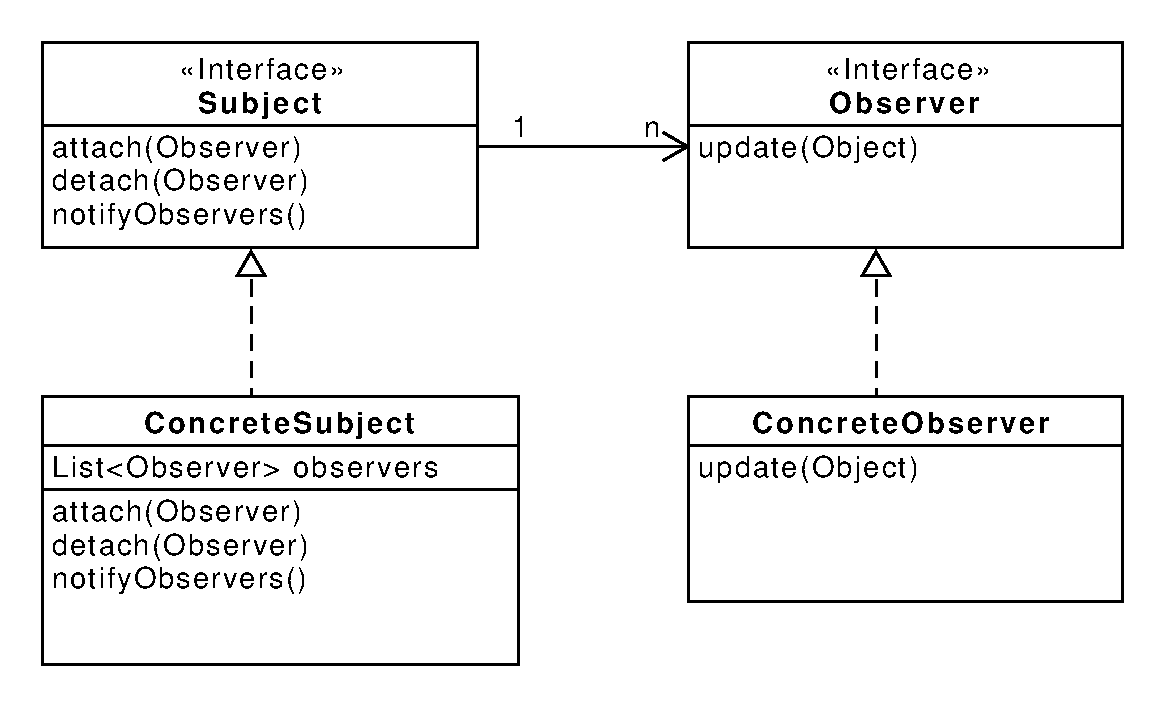
\includegraphics[width=0.7\textwidth]{./paper/observer/observer}
\caption{UML-Darstellung eines Observer-Pattern.}
\label{observerdiagramm}
\end{figure} 
